\section{What is Computation?}
\textbf{Computation} is the process of performing calculations, manipulating data, or executing a sequence of operations to solve problems or transform inputs into desired outputs. It encompasses both the theoretical and practical aspects of processing information.

\section{Computational Models: Theoretical Foundations}
A \textbf{computational model} is a mathematical or conceptual framework that defines how computation is carried out. For an arbitrary computing model, the following metaphoric expression has been proposed:
\begin{center}
    \textbf{computation = storage + transmission + processing}
\end{center}

\section{Four Fundamental Computational Models}

\subsection{Turing Machine (Alan Turing, 1936)}
\textbf{The Foundation of Algorithmic Computation}

\subsubsection{Core Characteristics}
\begin{itemize}
    \item \textbf{Style}: Imperative / mechanical model of computation
    \item \textbf{Core Idea}: A machine reads/writes symbols on an infinite tape with a finite set of rules
    \item \textbf{Representation}:
    \begin{itemize}
        \item Infinite tape divided into cells
        \item Head that can read/write and move left or right
        \item Finite state machine controlling transitions
    \end{itemize}
\end{itemize}

\subsubsection{Strengths and Limitations}
\textbf{Strengths}:
\begin{itemize}
    \item Canonical model for algorithmic computability
    \item Basis of the Church---Turing Thesis
    \item Directly models sequential execution
\end{itemize}

\textbf{Limitations}:
\begin{itemize}
    \item Low-level, not efficient
    \item Sequential by nature, doesn't capture parallelism well
\end{itemize}

\textbf{Example}: A Turing Machine can simulate any algorithm you'd run on a modern computer (given enough tape).

\subsection{Lambda Calculus (Alonzo Church, 1930s)}
\textbf{The Foundation of Functional Computation}

\subsubsection{Core Characteristics}
\begin{itemize}
    \item \textbf{Style}: Functional model of computation
    \item \textbf{Core Idea}: Everything is a function. Computation = function application + substitution
    \item \textbf{Representation}:
    \begin{itemize}
        \item Variables (\texttt{x})
        \item Function definitions (\texttt{$\lambda$x. expression})
        \item Function application (\texttt{(f x)})
    \end{itemize}
\end{itemize}

\subsubsection{Strengths and Limitations}
\textbf{Strengths}:
\begin{itemize}
    \item Basis of functional programming (Haskell, Lisp)
    \item Good for reasoning about higher-order functions, abstraction, recursion
\end{itemize}

\textbf{Limitations}:
\begin{itemize}
    \item Abstract and symbolic; not naturally tied to hardware
    \item Efficiency is not modeled, just computability
\end{itemize}

\textbf{Example}: Addition can be defined entirely in terms of functions (Church numerals).

\subsection{Cellular Automata (Stanislaw Ulam, John von Neumann, later Conway)}
\textbf{The Foundation of Distributed/Parallel Computation}

\subsubsection{Core Characteristics}
\begin{itemize}
    \item \textbf{Style}: Spatial / distributed model of computation
    \item \textbf{Core Idea}: Computation arises from simple local rules applied to a grid of cells over time
    \item \textbf{Representation}:
    \begin{itemize}
        \item Infinite (or finite) grid of cells
        \item Each cell has a finite state (e.g., alive/dead)
        \item Transition rules depend only on the local neighborhood
    \end{itemize}
\end{itemize}

\subsubsection{Strengths and Limitations}
\textbf{Strengths}:
\begin{itemize}
    \item Good for modeling parallel, distributed, physical systems
    \item Supports universal computation (Conway's Life is Turing-complete)
\end{itemize}

\textbf{Limitations}:
\begin{itemize}
    \item Not natural for symbolic or algebraic computation
    \item More suited for simulating dynamics
\end{itemize}

\textbf{Example}: Conway's \textit{Game of Life} shows how simple rules produce complex, even universal, behaviors.

\subsection{Biological Computation (Inspired by Nature)}
\textbf{The Foundation of Adaptive/Learning Computation}

\subsubsection{Core Characteristics}
Biological models are inspired by living systems and emphasize parallelism, adaptability, and learning.
\begin{itemize}
    \item \textbf{Learns from data} (training) rather than using fixed rules
    \item Massive parallelism and fault tolerance
    \item Self-organization and adaptation
    \item Pattern recognition and generalization
\end{itemize}

\subsubsection{Examples of Biological Computation}
\textbf{Neural Networks}:
\begin{itemize}
    \item Inspired by the brain's neurons and synapses
    \item Computation happens through weighted sums and nonlinear activations
    \item Foundation of modern AI (deep learning for vision, NLP, etc.)
\end{itemize}

\textbf{DNA Computing}:
\begin{itemize}
    \item Uses DNA strands and biochemical reactions to encode and solve problems
    \item Enables massive parallelism (billions of molecules interacting at once)
    \item Example: Adleman (1994) solved a small Hamiltonian Path problem with DNA
\end{itemize}

\textbf{Swarm Intelligence}:
\begin{itemize}
    \item Inspired by ants, bees, and bird flocks
    \item Simple agents interacting lead to complex global solutions
    \item Example: Ant Colony Optimization for shortest path problems
\end{itemize}

\section{Biological Neural Networks: Nature's Computational Model}
The following are key characteristics that make biological neural networks powerful computational systems:

\subsection{Characteristics of Biological Neural Networks}
\begin{itemize}
    \item \textbf{Highly interconnected:} Neurons form a complex web of connections
    \item \textbf{Robustness and Fault Tolerance:} The decay of nerve cells does not affect the overall function of the network significantly
    \item \textbf{Flexibility:} The ability to reorganize and adapt to new situations
    \item \textbf{Handling incomplete information:} Ability to infer appropriate outputs even when some inputs are missing or noisy
    \item \textbf{Parallel processing:} Multiple neurons can process information simultaneously
\end{itemize}
\subsection{Neuron Structure}
\begin{figure}[h!]
\centering
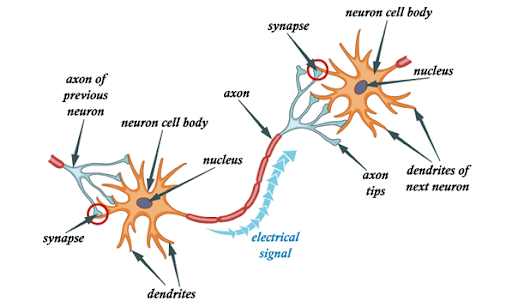
\includegraphics[width=0.8\textwidth]{biological_neuron.png}
\caption{Structure of a biological neuron.}
\end{figure}
\subsection{Neuron Structure and Components}
\begin{itemize}
    \item \textbf{Fundamental unit}: neuron (cell body / soma, dendrites, axon, synapses)
    \item \textbf{Dendrites} receive inputs; \textbf{axon} transmits output and branches to many synapses (often thousands)
    \item \textbf{Synapse}: junction between axon terminal and target cell
    \item \textbf{Synaptic junctions} form between presynaptic axon terminals and postsynaptic dendrites or the cell body
\end{itemize}

\subsubsection{Typical Sizes}
\begin{itemize}
    \item soma $\sim$ 10--80 $\mu$m
    \item synaptic gap $\sim$ 200 nm
    \item neuron length from 0.01 mm to 1 m
\end{itemize}

\subsection{Signal Transmission and Firing}
\begin{itemize}
    \item \textbf{Resting potential} $\sim$ -70 mV; depolarization above threshold (roughly $\sim$10 mV) triggers firing
    \item \textbf{Action potentials} are all-or-none pulses sent down the axon; information is encoded in firing rate ($\sim$1--100 Hz)
    \item \textbf{Propagation speed} in brain tissue $\sim$ 0.5--2 m/s; synaptic transmission delay $\sim$ 0.5 ms
    \item After firing the membrane recovers (\textbf{refractory period}); synaptic effects decay with time constant $\sim$5--10 ms
\end{itemize}

\subsection{Synapses: Chemistry and Types}
\begin{itemize}
    \item \textbf{Transmission} across synapse is chemical: neurotransmitters released from presynaptic terminal
    \item \textbf{Postsynaptic effect} can be excitatory (depolarizing) or inhibitory (hyperpolarizing)
    \item All endings of a given axon are typically either excitatory or inhibitory
    \item \textbf{Synaptic strength} depends on activity and can change over time (basis for learning)
\end{itemize}



\subsection{Plasticity and Learning}
Active synapses that repeatedly contribute to postsynaptic firing tend to strengthen; inactive ones weaken. \textbf{Hebb's rule} ("cells that fire together, wire together") describes this activity-dependent plasticity. Continuous modification of synaptic strengths underlies learning and memory formation.

\section{Artificial Neural Networks}
\subsection{Introduction: From Biology to Computation}
Artificial Neural Networks (ANNs) represent one of the most successful attempts to harness the computational principles observed in biological neural systems for solving complex problems.

\subsection{The Abstract Neuron: Building Block of Intelligence}
The output of a neuron can be expressed as:
\[ Y = f\left(\sum_{i=1}^{n} W_i X_i + b\right) = f(\mathbf{W}^T \mathbf{X} + b)\]
Where:
\begin{itemize}
    \item \(Y\): Output of the neuron
    \item \(f\): Activation function (primitive function that introduces non-linearity)
    \item \(W_i\): Weight associated with input \(i\) (learnable parameter)
    \item \(X_i\): Value of input \(i\)
    \item \(b\): Bias term (learnable parameter that shifts the activation function)
    \item \(\mathbf{W} = [W_1, W_2, \ldots, W_n]^T\): Weight vector
    \item \(\mathbf{X} = [X_1, X_2, \ldots, X_n]^T\): Input vector
\end{itemize}

\subsubsection{Mathematical Foundation: Linear Combination and Affine Transformation}
The computation \(\mathbf{W}^T \mathbf{X} + b\) represents an \textbf{affine transformation} of the input space. This can be broken down as:
\begin{enumerate}
    \item \textbf{Linear transformation}: \(\mathbf{W}^T \mathbf{X}\) scales and rotates the input vector
    \item \textbf{Translation}: Adding bias \(b\) shifts the result by a constant
\end{enumerate}

The activation function \(f\) then introduces non-linearity, enabling the neuron to model complex, non-linear relationships between inputs and outputs.

\section{Activation Functions: Mathematical Properties}
Activation functions are crucial for introducing non-linearity into neural networks. Different activation functions have distinct mathematical properties that affect learning dynamics.

\subsection{Common Activation Functions}
\subsubsection{Step Function (Heaviside)}
\[\phi(z) = \begin{cases} 1 & \text{if } z \geq 0 \\ 0 & \text{if } z < 0 \end{cases}\]
\textbf{Properties}: Non-differentiable, binary output, historically important for perceptron.

\subsubsection{Sigmoid Function}
\[\sigma(z) = \frac{1}{1 + e^{-z}}\]
\textbf{Properties}:
\begin{itemize}
    \item Smooth, differentiable: \(\sigma'(z) = \sigma(z)(1 - \sigma(z))\)
    \item Range: \((0, 1)\)
    \item Problem: Vanishing gradients for large \(|z|\)
\end{itemize}

\subsubsection{Hyperbolic Tangent}
\[\tanh(z) = \frac{e^z - e^{-z}}{e^z + e^{-z}} = 2\sigma(2z) - 1\]
\textbf{Properties}:
\begin{itemize}
    \item Range: \((-1, 1)\)
    \item Zero-centered output
    \item Derivative: \(\tanh'(z) = 1 - \tanh^2(z)\)
\end{itemize}

\subsubsection{Rectified Linear Unit (ReLU)}
\[\text{ReLU}(z) = \max(0, z)\]
\textbf{Properties}:
\begin{itemize}
    \item Computationally efficient
    \item Alleviates vanishing gradient problem
    \item Non-differentiable at \(z = 0\)
    \item Can suffer from "dying ReLU" problem
\end{itemize}

\subsection{Mathematical Requirements for Activation Functions}
For universal approximation, activation functions should be:
\begin{enumerate}
    \item \textbf{Non-linear}: Otherwise, multiple layers collapse to a single linear transformation
    \item \textbf{Differentiable}: Enables gradient-based optimization (almost everywhere is sufficient)
    \item \textbf{Monotonic}: Helps with optimization landscape (not strictly required)
    \item \textbf{Bounded or unbounded}: Different properties affect convergence behavior
\end{enumerate}

\subsection{Neural Networks as Function Approximators}
With sufficient neurons and appropriate activation functions, neural networks can approximate any continuous function to arbitrary precision.

\subsubsection{Universal Approximation Theorem}
\textbf{Theorem (Cybenko, 1989; Hornik, 1991)}: Let \(\phi\) be a continuous sigmoid-type function. Then finite sums of the form:
\[F(x) = \sum_{j=1}^{N} \alpha_j \phi(y_j^T x + \theta_j)\]
are dense in \(C(I_n)\), the space of continuous functions on the unit hypercube \(I_n = [0,1]^n\).

\subsubsection{Implications}
\begin{itemize}
    \item \textbf{Existence}: There exists a neural network that can approximate any continuous function
    \item \textbf{No constructive proof}: Doesn't tell us how to find the network
    \item \textbf{Width vs. Depth}: Original theorem about width; depth can be more efficient
    \item \textbf{Approximation vs. Learning}: Says nothing about learnability from data
\end{itemize}

\subsubsection{Modern Extensions}
\begin{itemize}
    \item \textbf{ReLU networks}: Also have universal approximation properties
    \item \textbf{Deep vs. Wide}: Deep networks can be exponentially more efficient than wide ones
    \item \textbf{Smooth functions}: Require fewer neurons than general continuous functions
\end{itemize}

\section{Artificial Neural Networks: From Theory to Implementation}

\subsection{Fundamental Architecture: Primitive Functions and Composition Rules}
To understand artificial neural networks, we must first examine their core computational elements. Every computational model requires:
\begin{enumerate}
    \item \textbf{Primitive Functions}: Basic operations that cannot be decomposed further
    \item \textbf{Composition Rules}: Ways to combine primitive functions to create complex behaviors
\end{enumerate}

\subsubsection{Primitive Functions in Neural Networks}
In artificial neural networks, \textbf{primitive functions are located in the nodes (neurons) of the network}. Each node implements a specific mathematical transformation that processes incoming information and produces an output.

\subsubsection{Composition Rules in Neural Networks}
The \textbf{composition rules are contained implicitly in}:
\begin{itemize}
    \item \textbf{Interconnection pattern of the nodes}: How neurons are connected determines information flow
    \item \textbf{Synchrony or asynchrony of information transmission}: Whether neurons update simultaneously or in sequence
    \item \textbf{Presence or absence of cycles}: Whether information can flow in loops (recurrent networks) or only forward (feedforward networks)
\end{itemize}

This differs fundamentally from traditional computing models:

\begin{table}[h!]
\centering
\begin{tabular}{|l|l|l|}
\hline
\textbf{Computing Model} & \textbf{Primitive Functions} & \textbf{Composition Rules} \\
\hline
\textbf{von Neumann Processor} & Machine instructions & Program sequence + control flow \\
& (ADD, MOVE, JUMP) & \\
\hline
\textbf{Artificial Neural Networks} & Neuron activation functions & Network topology + connection \\
& & weights + timing \\
\hline
\end{tabular}
\caption{Comparison of primitive functions and composition rules across computing models.}
\end{table}

\subsection{Neural Networks as Function Approximators}

\subsubsection{Networks of Primitive Functions}
\textbf{Artificial neural networks are nothing but networks of primitive functions.} Each node transforms its input into a precisely defined output, and the combination of these transformations creates complex computational behaviors.

\subsubsection{The Network Function}
Consider a neural network that takes inputs $(x, y, z)$ and produces an output through nodes implementing primitive functions $f_1, f_2, f_3, f_4$. The network can be thought of as implementing a \textbf{network function} $\phi$:
\[\phi(x, y, z) = f_4(a_4 \cdot f_3(a_3 \cdot f_2(a_2 \cdot f_1(a_1 \cdot x))) + \ldots)\]
Where $a_1, a_2, \ldots, a_5$ are the weights of the network. \textbf{Different selections of weights produce different network functions.}

\subsubsection{Three Critical Elements}
Different models of artificial neural networks differ mainly in three fundamental aspects:
\begin{enumerate}
    \item \textbf{Structure of the Nodes}
    \begin{itemize}
        \item Choice of activation function (sigmoid, ReLU, tanh, etc.)
        \item Input integration method (weighted sum, product, etc.)
        \item Presence of bias terms
    \end{itemize}
    \item \textbf{Topology of the Network}
    \begin{itemize}
        \item Feedforward vs. recurrent connections
        \item Number of layers and neurons per layer
        \item Connection patterns (fully connected, sparse, convolutional)
    \end{itemize}
    \item \textbf{Learning Algorithm}
    \begin{itemize}
        \item Method for finding optimal weights
        \item Supervised vs. unsupervised vs. reinforcement learning
        \item Optimization techniques (gradient descent, evolutionary algorithms)
    \end{itemize}
\end{enumerate}

\subsection{Function Approximation: The Classical Problem}

\subsubsection{Historical Context}
Function approximation is a classical problem in mathematics: \textbf{How can we reproduce a given function $F : \mathbb{R} \rightarrow \mathbb{R}$ either exactly or approximately using a given set of primitive functions?}

Traditional approaches include:
\begin{itemize}
    \item \textbf{Polynomial approximation}: Using powers of $x$ (Taylor series)
    \item \textbf{Fourier approximation}: Using trigonometric functions (sine and cosine)
    \item \textbf{Spline approximation}: Using piecewise polynomials
\end{itemize}

\subsubsection{Neural Networks as Universal Approximators}
Neural networks provide a revolutionary approach to function approximation:

\textbf{Key Insight}: With sufficient neurons and appropriate activation functions, neural networks can approximate any continuous function to arbitrary precision (Universal Approximation Theorem).

\subsubsection{Advantages of Neural Network Approximation}
\begin{enumerate}
    \item \textbf{Adaptive}: Networks learn the approximation from data rather than requiring explicit mathematical formulation
    \item \textbf{Flexible}: Can handle high-dimensional inputs and complex, non-linear relationships
    \item \textbf{Robust}: Can generalize to unseen data and handle noise
    \item \textbf{Parallel}: Multiple neurons can process different aspects of the input simultaneously
\end{enumerate}

\subsection{Learning from Data: The Key Difference}
The main difference between Taylor or Fourier series and artificial neural networks is, however, that \textbf{the function F to be approximated is given not explicitly but implicitly through a set of input-output examples.} We know F only at some points but we want to generalize as well as possible. This means that we try to adjust the parameters of the network in an optimal manner to reflect the information known and to extrapolate to new input patterns which will be shown to the network afterwards. This is the task of the learning algorithm used to adjust the network's parameters.

\subsubsection{Classical Series vs. Neural Networks: A Fundamental Distinction}

\textbf{Classical Mathematical Series (Taylor/Fourier):}
\begin{itemize}
    \item \textbf{Explicit Function Definition}: The function $F(x)$ is mathematically defined and known
    \item \textbf{Analytical Coefficients}: Series coefficients can be computed directly using calculus
    \begin{itemize}
        \item Taylor: $a_n = F^{(n)}(x_0)/n!$ (nth derivative at expansion point)
        \item Fourier: $a_n, b_n$ computed via integration over the function's period
    \end{itemize}
    \item \textbf{Perfect Representation}: Given enough terms, the series can represent the function exactly
    \item \textbf{No Learning Required}: Coefficients are determined mathematically, not learned
\end{itemize}

\textbf{Artificial Neural Networks:}
\begin{itemize}
    \item \textbf{Implicit Function Definition}: The function F is unknown but represented by data points
    \item \textbf{Learned Parameters}: Network weights and biases are learned from examples
    \item \textbf{Approximation from Samples}: Must generalize from finite training data to unknown inputs
    \item \textbf{Adaptive Learning}: Parameters adjust through iterative optimization algorithms
\end{itemize}

\subsubsection{Mathematical Formulation of the Learning Problem}
Given a training dataset \(\mathcal{D} = \{(\mathbf{x}_i, y_i)\}_{i=1}^{m}\), we seek to find parameters \(\boldsymbol{\theta}\) that minimize the empirical risk:
\[\mathcal{R}_{\text{emp}}(\boldsymbol{\theta}) = \frac{1}{m} \sum_{i=1}^{m} L(f(\mathbf{x}_i; \boldsymbol{\theta}), y_i)\]

where:
\begin{itemize}
    \item \(L(\cdot, \cdot)\): Loss function measuring prediction error
    \item \(f(\mathbf{x}; \boldsymbol{\theta})\): Neural network function with parameters \(\boldsymbol{\theta}\)
    \item Goal: Minimize true risk \(\mathcal{R}(\boldsymbol{\theta}) = \mathbb{E}_{(\mathbf{x},y) \sim P}[L(f(\mathbf{x}; \boldsymbol{\theta}), y)]\)
\end{itemize}

\subsubsection{Generalization Gap}
The fundamental challenge is the generalization gap:
\[\text{Generalization Gap} = \mathcal{R}(\boldsymbol{\theta}) - \mathcal{R}_{\text{emp}}(\boldsymbol{\theta})\]

This gap can be controlled through:
\begin{enumerate}
    \item \textbf{Regularization}: Adding penalty terms to control model complexity
    \item \textbf{Cross-validation}: Using held-out data to estimate generalization performance
    \item \textbf{Early stopping}: Halting training before overfitting occurs
    \item \textbf{Data augmentation}: Artificially increasing training set size
\end{enumerate}

\section{Computational Complexity in Neural Networks}
\subsection{Forward Pass Complexity}
For a neural network with \(L\) layers, where layer \(l\) has \(n_l\) neurons:
\begin{itemize}
    \item \textbf{Matrix multiplication}: \(O(n_{l-1} \times n_l)\) for each layer
    \item \textbf{Total forward pass}: \(O(\sum_{l=1}^{L} n_{l-1} \times n_l)\)
    \item \textbf{Activation functions}: \(O(n_l)\) per layer (typically much smaller than matrix operations)
\end{itemize}

\subsection{Backward Pass Complexity (Backpropagation)}
\begin{itemize}
    \item \textbf{Gradient computation}: Same order as forward pass \(O(\sum_{l=1}^{L} n_{l-1} \times n_l)\)
    \item \textbf{Parameter updates}: \(O(\text{total parameters})\)
    \item \textbf{Memory complexity}: \(O(\text{total activations})\) to store intermediate values
\end{itemize}

\subsection{Scalability Considerations}
\begin{itemize}
    \item \textbf{Batch processing}: Process multiple examples simultaneously for efficiency
    \item \textbf{Parallelization}: Matrix operations are highly parallelizable on GPUs
    \item \textbf{Memory-computation tradeoff}: Can reduce memory by recomputing activations
\end{itemize}
